% Copyright 2020-2022 Robert Bosch GmbH

% Licensed under the Apache License, Version 2.0 (the "License");
% you may not use this file except in compliance with the License.
% You may obtain a copy of the License at

% http://www.apache.org/licenses/LICENSE-2.0

% Unless required by applicable law or agreed to in writing, software
% distributed under the License is distributed on an "AS IS" BASIS,
% WITHOUT WARRANTIES OR CONDITIONS OF ANY KIND, either express or implied.
% See the License for the specific language governing permissions and
% limitations under the License.

\hypertarget{webapp-architecture}{%
\section{WebApp Architecture:}\label{webapp-architecture}}

The WebApp application includes:
\begin{itemize}
   \item The database: mysql is used - which contains on the test execution 
         results. For detail of all tables in databse, please refer the 
         \href{https://github.com/test-fullautomation/testresultwebapp/blob/
         develop/TestResultWebApp/mysql_server/datamodel/datamodel.svg}{database
         model}.
   \item Active Directory: for the authentication.
   \item Web server: which is hosted for static data and run the nodejs 
         application for the dynamic data (API call).
\end{itemize}

Please refer below architecture for more detail:

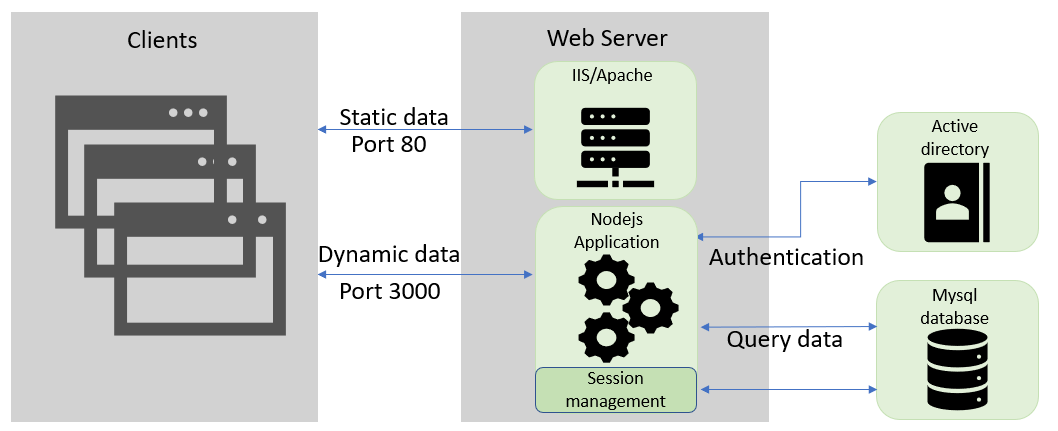
\includegraphics[width=1\linewidth]{./pictures/Architechture.png}

\hypertarget{import-data}{%
\section{Import Data:}\label{import-data}}

The data which will be visualized on webapp are get directly from the database.
So that the test execution result information should be transformed first 
follows \href{https://github.com/test-fullautomation/testresultwebapp/blob/
develop/TestResultWebApp/mysql_server/datamodel/datamodel.svg}
{the defined database model} then import to database.

We have already provided the \href{https://github.com/test-fullautomation/
robotframework-testresultwebapptool}{RobotResults2DB} which helps to import the
\rfwcore\ result file(s) \emph{output.xml} to the database of testresult webapp.

You will need to provide only the \rfwcore\ result file(s) and database's 
information, that import tool will parse the test execution result information 
and interact with provided database to import the according data.

Please refer \href{https://github.com/test-fullautomation/
robotframework-testresultwebapptool#usage}{RobotResults2DB's usage} and 
\href{https://github.com/test-fullautomation/robotframework-
testresultwebapptool/blob/develop/RobotResults2DB/RobotResults2DB.pdf}
{its document} for more detail.


\hypertarget{data-visualization}{%
\section{Data Visualization:}\label{data-visualization}}

\hypertarget{main-menu}{%
\subsection{Main menu:}\label{main-menu}}
WebApp provides the main menu for user to select the specific branch, 
project/variant and software version to be displayed.

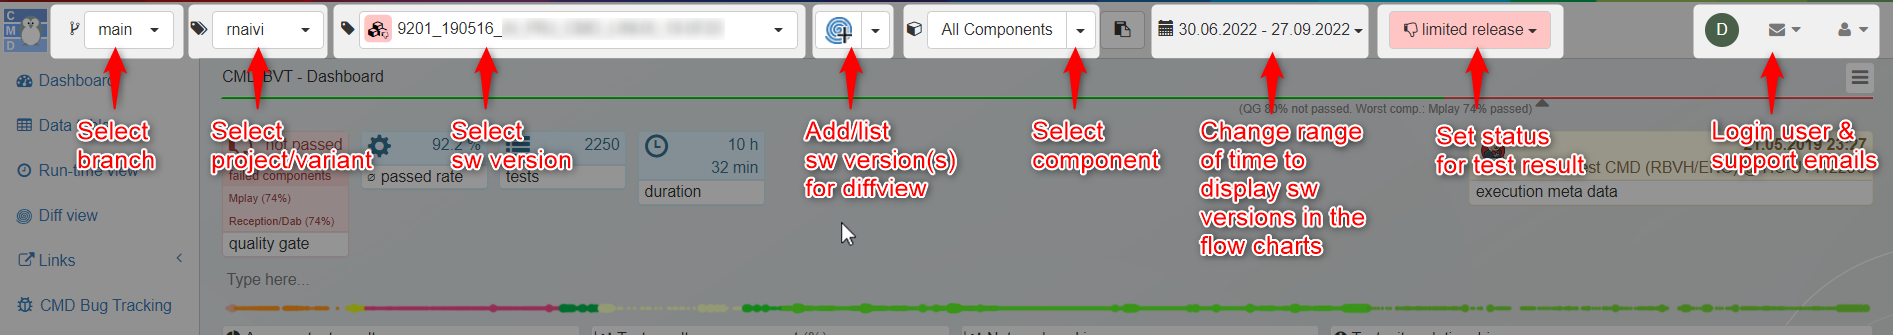
\includegraphics[width=1\linewidth]{./pictures/main-menu.png}

\hypertarget{dashboard-view}{%
\subsection{Dashboard View:}\label{dashboard-view}}
Dashboard view does not only provide an overview of test execution results but 
also shows the correlation betweeen components within the result 
and relationship with other test execution results.

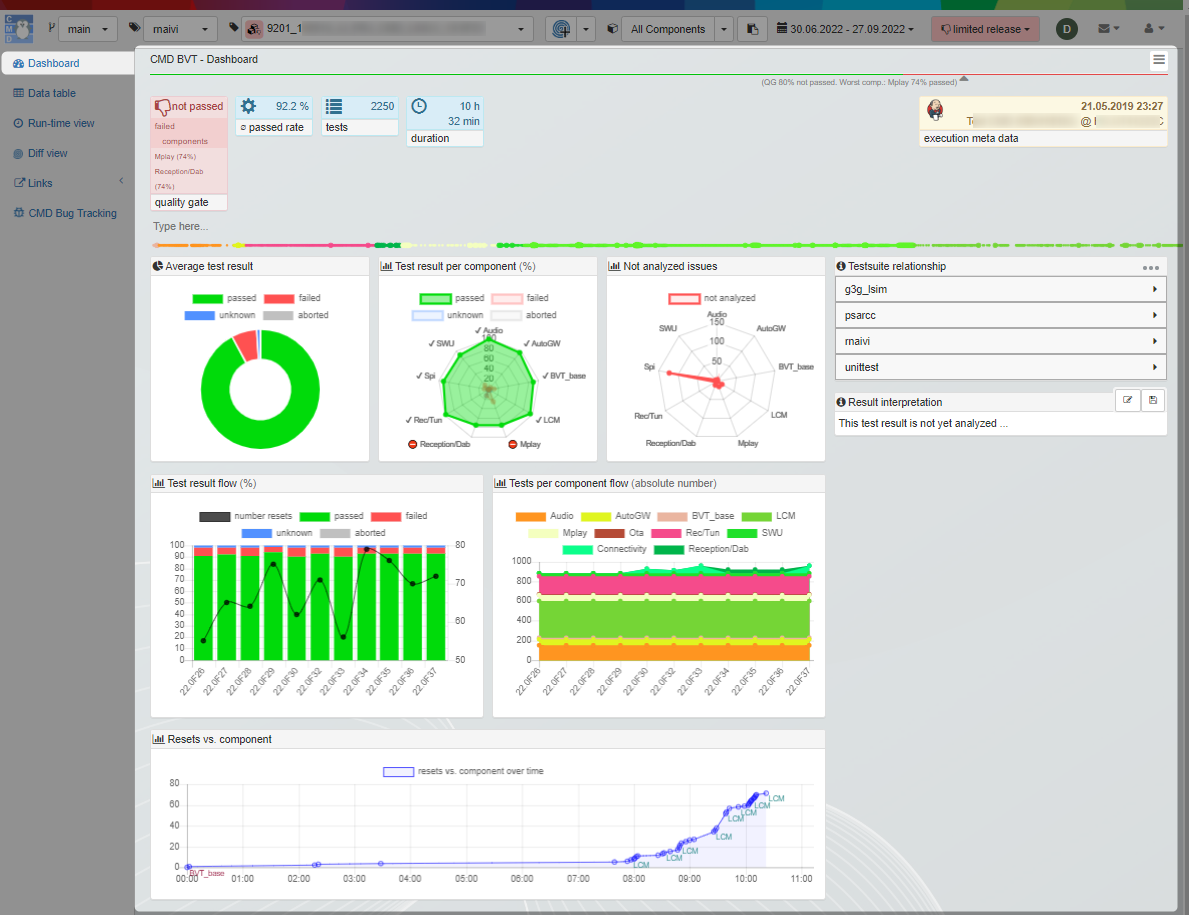
\includegraphics[width=1\linewidth]{./pictures/view_dashboard.png}

\subsubsection{Result overview:}
On the top left conner of the Dashboard view, there is test execution result 
statistics:

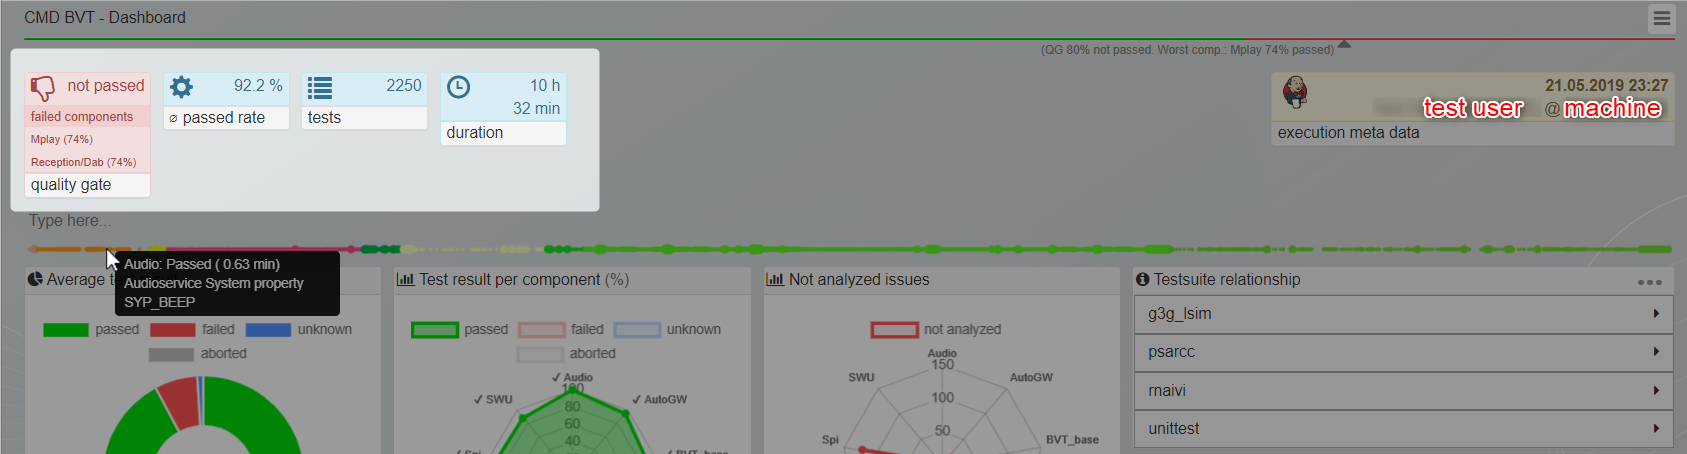
\includegraphics[width=1\linewidth]{./pictures/dashboard/result_statistics.png}

Which contains:
\begin{itemize}
   \item Overrall status.
   \item Passed rate.
   \item Total executed test cases.
   \item Test execution duration.
\end{itemize}

On other right-hand side, there is information about execution environemnt:

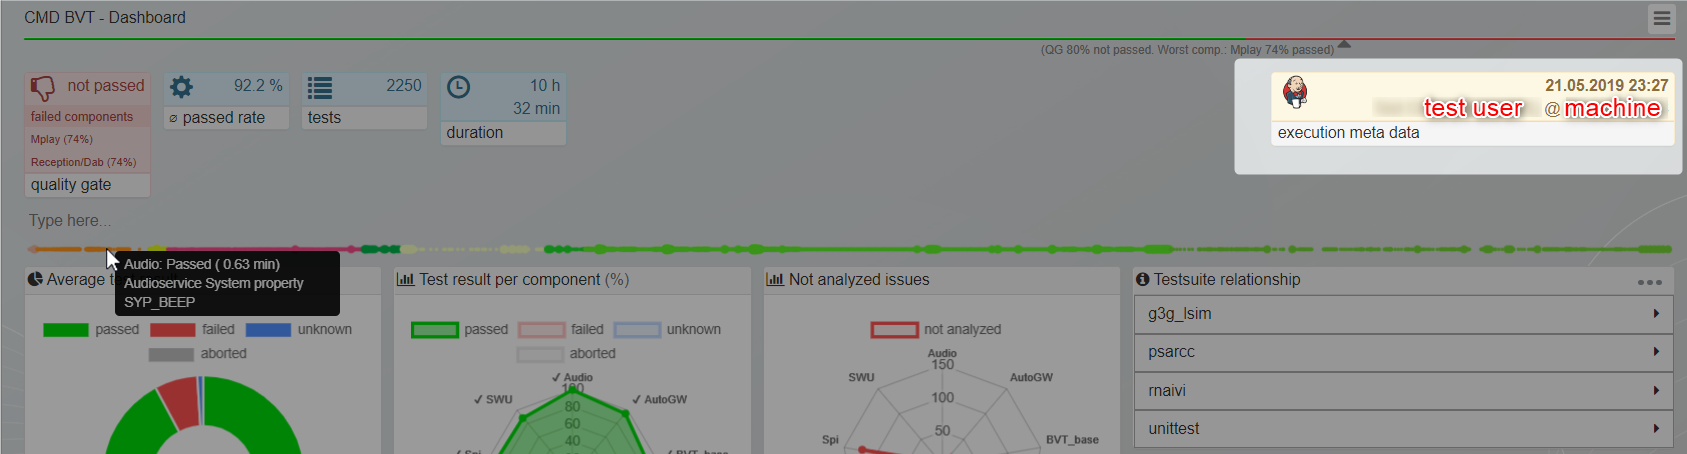
\includegraphics[width=1\linewidth]{./pictures/dashboard/result_environment.png}
\begin{itemize}
   \item Execution time
   \item Test machine
   \item Test user
   \item Jenkins link (embedded URL in the Jenkins's icon)
\end{itemize}

Below them is the test execution result timeline:

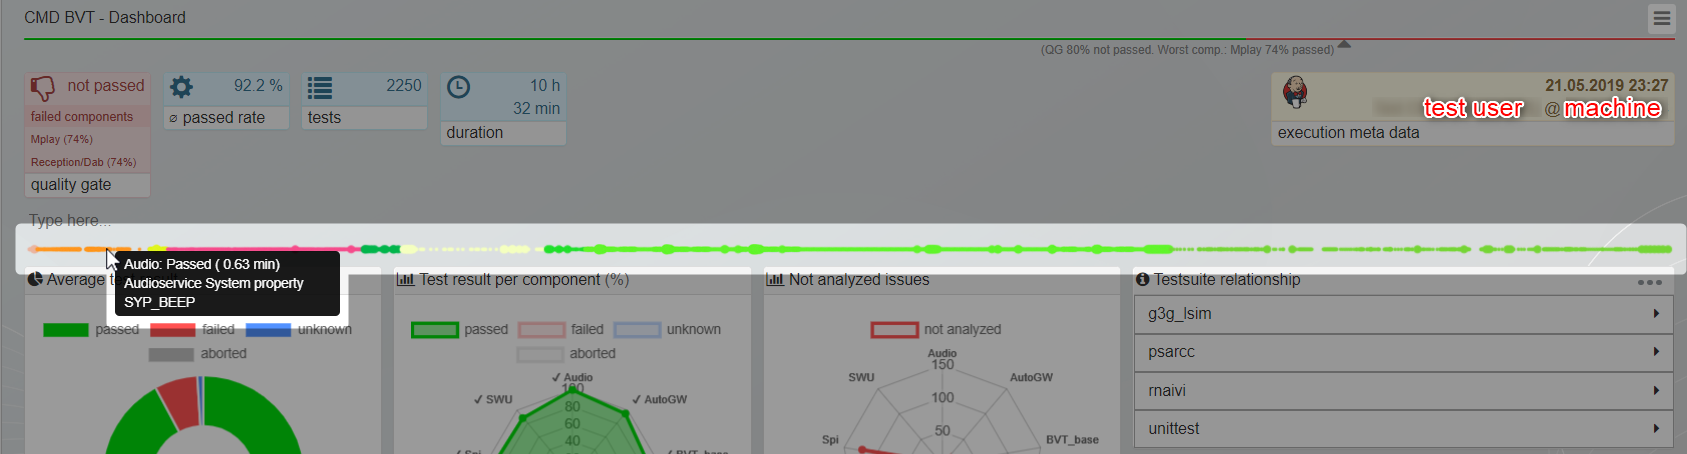
\includegraphics[width=1\linewidth]{./pictures/dashboard/result_timeline.png}

It provides:
\begin{itemize}
   \item The timeline of the executed test cases by components (different color).
   \item How much time is consumed by the individual test case by the distance 
         to the next test on time line or the detail pop-up when hovering on the 
         dot of the timeline.
   \item Test status result: small dot for passed status and big dot for others.
\end{itemize}


The next \textbf{Average test result} chart will give you the detail of test 
result with the percentage (number of test cases will be showed when mousing 
over the pie chart) of each result status (\ifpassed{Passed}, \iffailed{Failed}, 
\ifunknown{Unknown} or \ifaborted{Aborted}) in the execution. 

So that, you can qualify this test execution result is good or not.

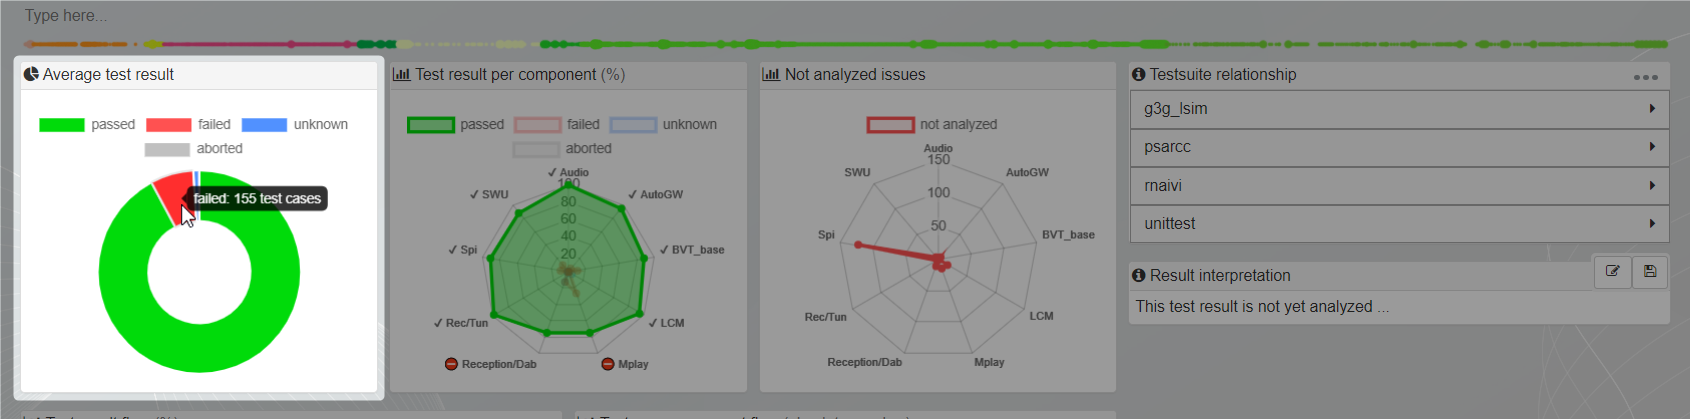
\includegraphics[width=1\linewidth]
{./pictures/dashboard/chart_average_test_result.png}

\subsubsection{Component's correlation:}
The next charts will help you to get the correlation between components within
the test result, so that you can know which component(s) is impacted to the test
result.

- \textbf{Test result per component} chart: provides the passed percentages of 
all components within test results and the quality of them compare the 
expectated quality gate (default: 80\%).\\
So that, you can justify the impact of component to the whole test execution
result.

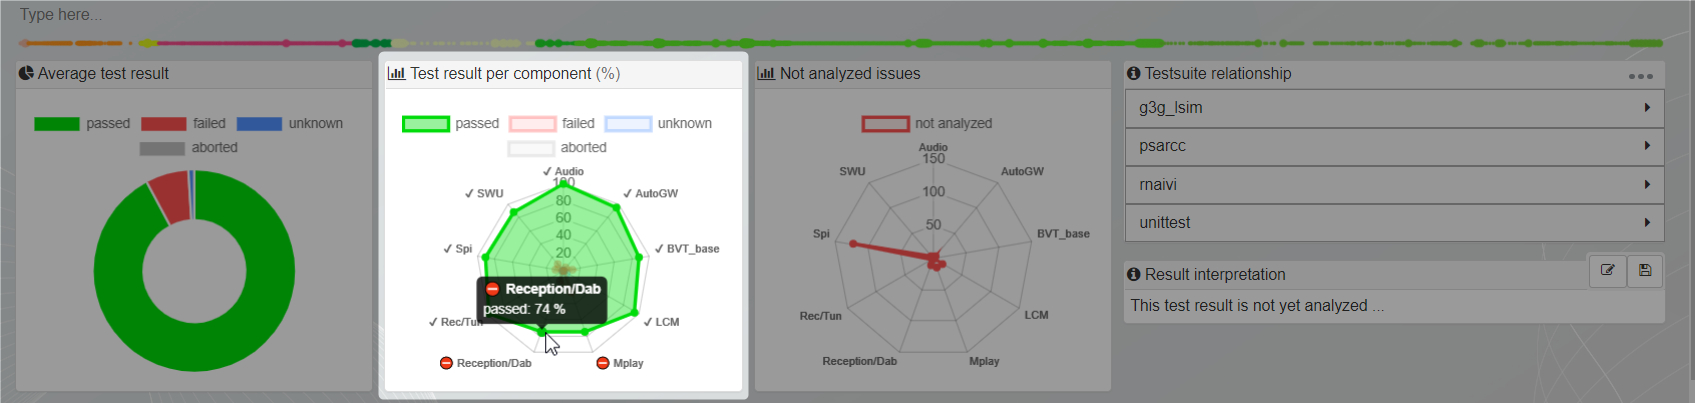
\includegraphics[width=1\linewidth]
{./pictures/dashboard/chart_test_result_per_component.png}


- \textbf{Not analyzed issues} chart: you can known how many test cases of 
components are issued without any analysis. 

So that, you can have the appropriate actions to the component team.

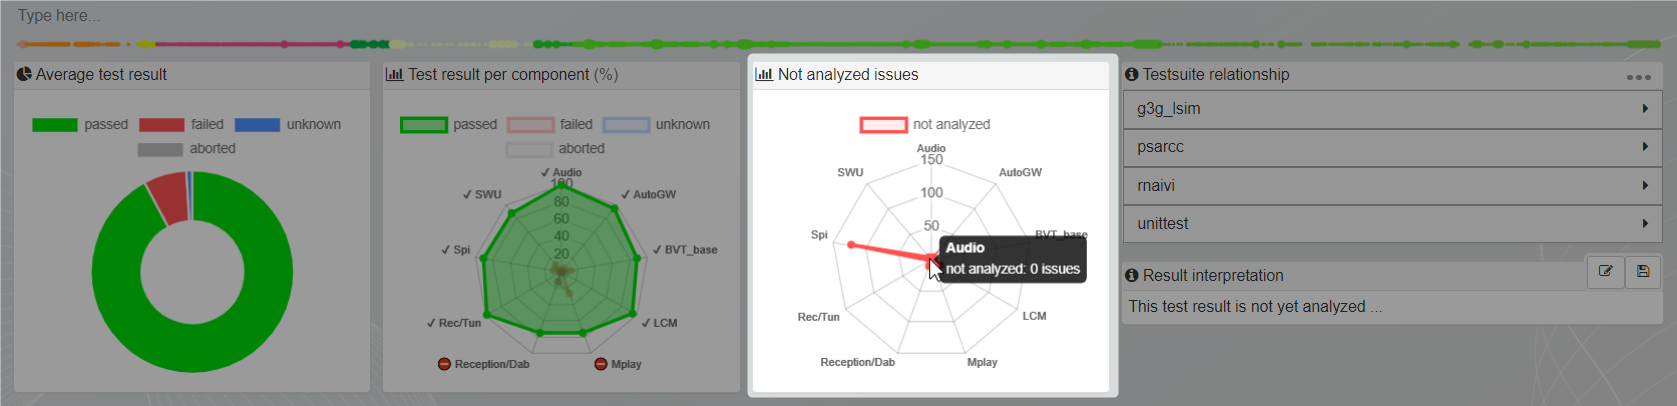
\includegraphics[width=1\linewidth]
{./pictures/dashboard/chart_not_analyzed_issues.png}

\subsubsection{Relationships with other test execution results:}

- \textbf{Testsuite relationship}: will let you know all the related test 
results (grouped by project/variant) of the the current selected version.

So that you can quickly go to the related test results to have the comparison
about the quality of the selected version across the projects/variants.

For example: the selected version have been executed for 4 projects/variants:
\emph{g3g\_lsim}, \emph{psarcc}, \emph{rnaivi} and \emph{unittest}. Each 
variant (except the \emph{unittest}) has 2 test results 
(one for the smoke test and one for the whole test execution result).

Then, all the related test execution results will be displayed as below:

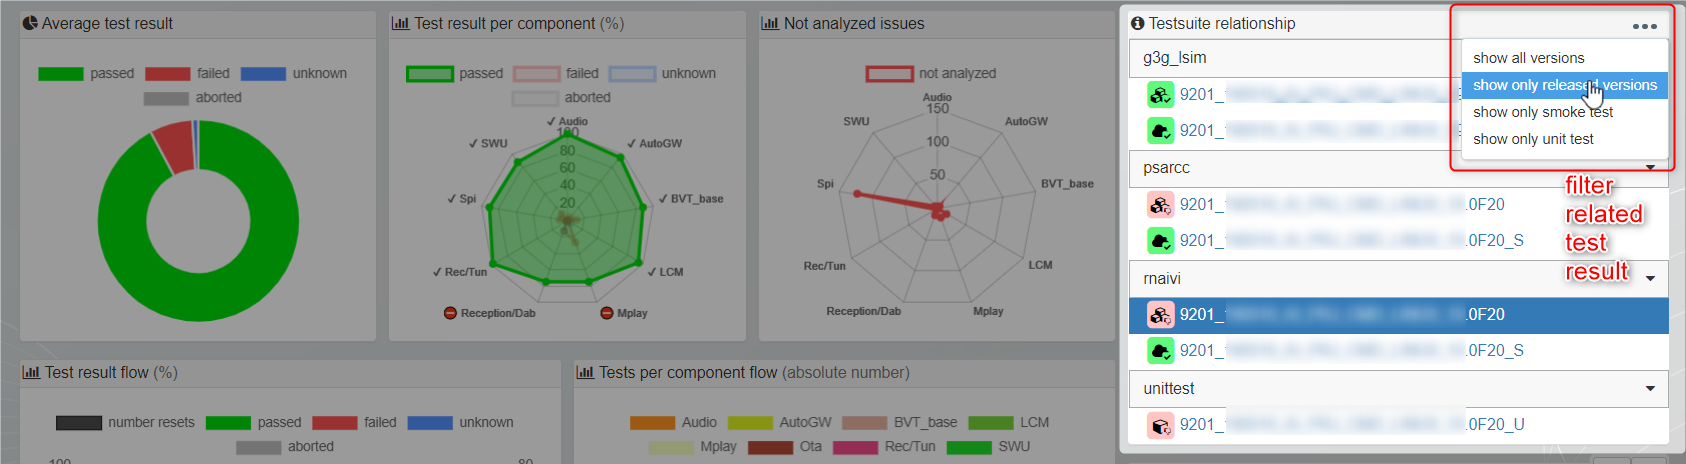
\includegraphics[width=1\linewidth]
{./pictures/dashboard/testsuite_relationship.png}

There is the context menu (\textbf{...}) that allow you to filter the related 
test results.

- \textbf{Test result flow} chart: provides the picture of quality change 
(percentages of each status) between versions. 

So that, you can understand the quality of testing software is being improved 
or vice versa.

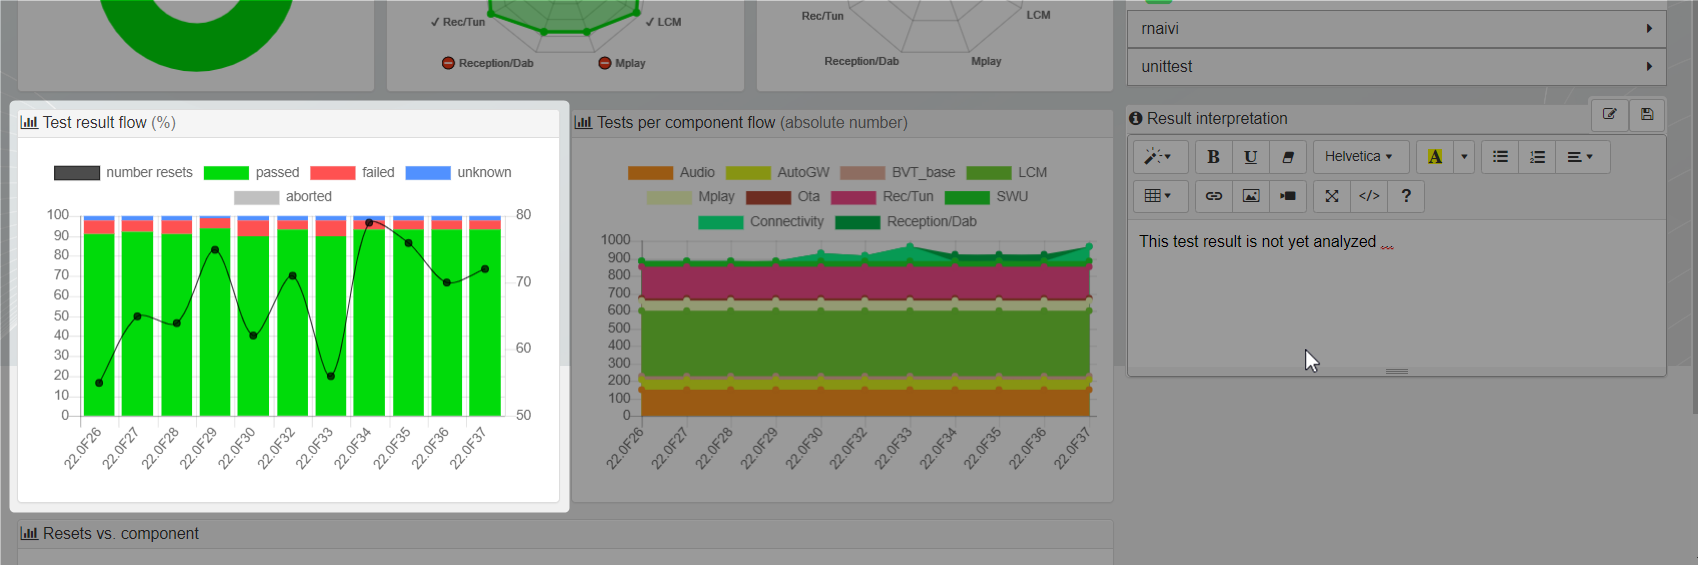
\includegraphics[width=1\linewidth]{./pictures/dashboard/chart_test_result_flow.png}

- \textbf{Tests per component flow} chart: provides the change of number test
cases per component between versions.

You can aware the number of test cases per component and how many test cases are
added or removed (per component or the whole test result) from those versions.

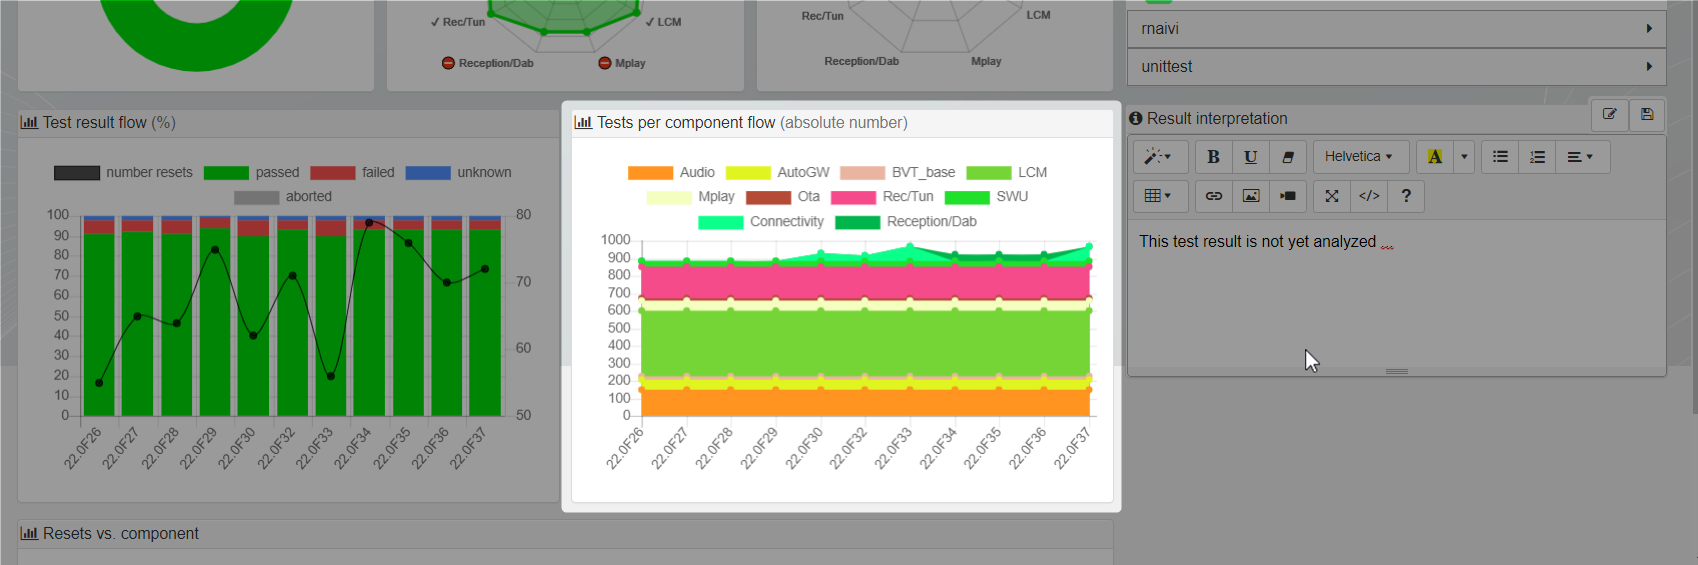
\includegraphics[width=1\linewidth]
{./pictures/dashboard/chart_tests_per_component_flow.png}

\begin{boxhint}{Notice}
The versions which are displayed in \textbf{Test result flow} and 
\textbf{Tests per component flow} charts are the executed test results within 
the selected range of time in 
\hyperref[main-menu]{the main menu} (default is \textbf{Last 90 Days}).
\end{boxhint}

\subsubsection{Result interpretation:}
You can give more information, analyze, take note, ... about the execution
result by leaving comments in the \textbf{Result interpretation} section.

As soon as the comment(s) is saved, that information will be updated to 
the database. So that, other users who browse to this test result can see
the analysis/comment for reference.

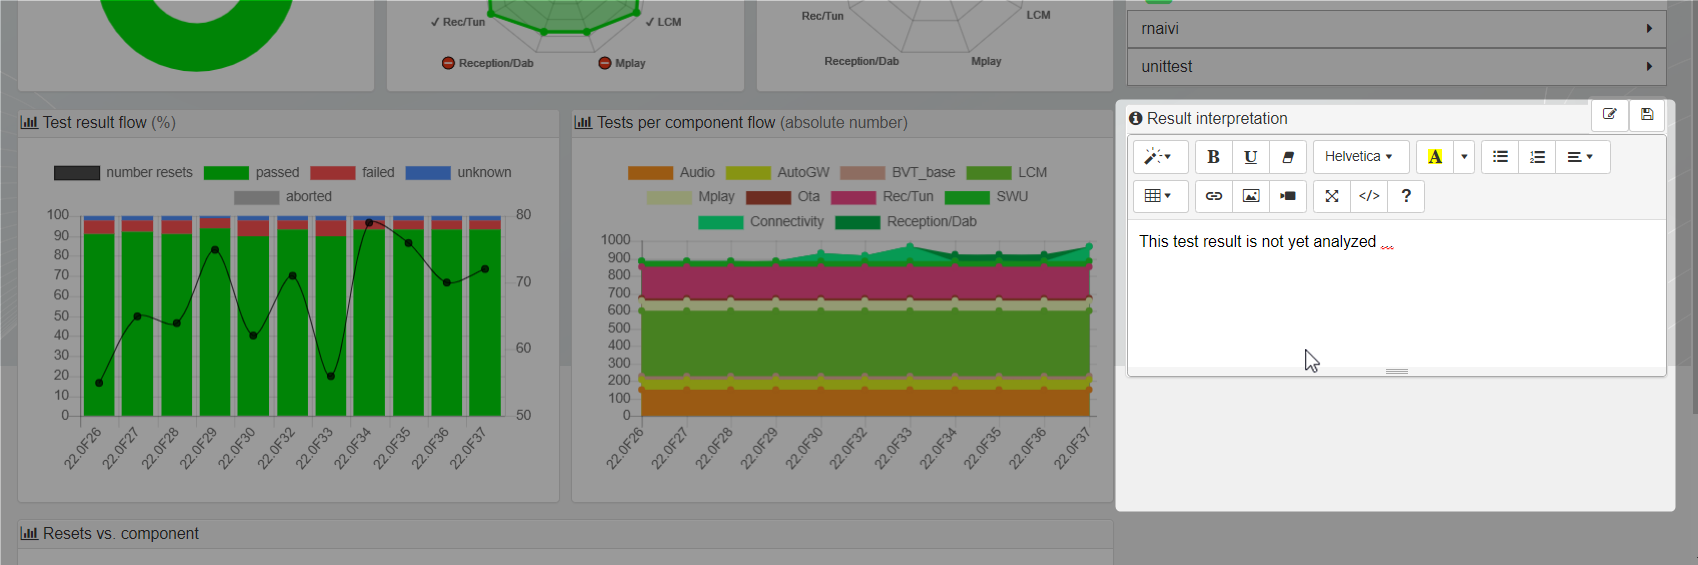
\includegraphics[width=1\linewidth]
{./pictures/dashboard/result_interpretation.png}

\subsubsection{Resets vs. component:}

The \textbf{Resets vs. component} chart will helps you to know the interaction
of component with the DUT (device under test) by providing the the reset counter
per component during the execution.

You can have awareness that:
\begin{itemize}
   \item When DUT has been reset.
   \item Which component has reset the DUT.
   \item How many reset has been done during each component and the whole
         test execution.
\end{itemize}

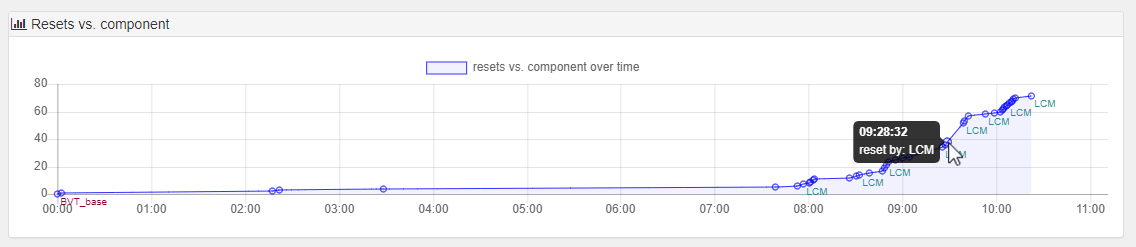
\includegraphics[width=1\linewidth]
{./pictures/dashboard/reset_vs_component.png}

\hypertarget{datatable-view}{%
\subsection{DataTable View}\label{datatable-view}}

Datatable view provides the table which contains the detail information of each
test case (grouped by component) within the test execution.

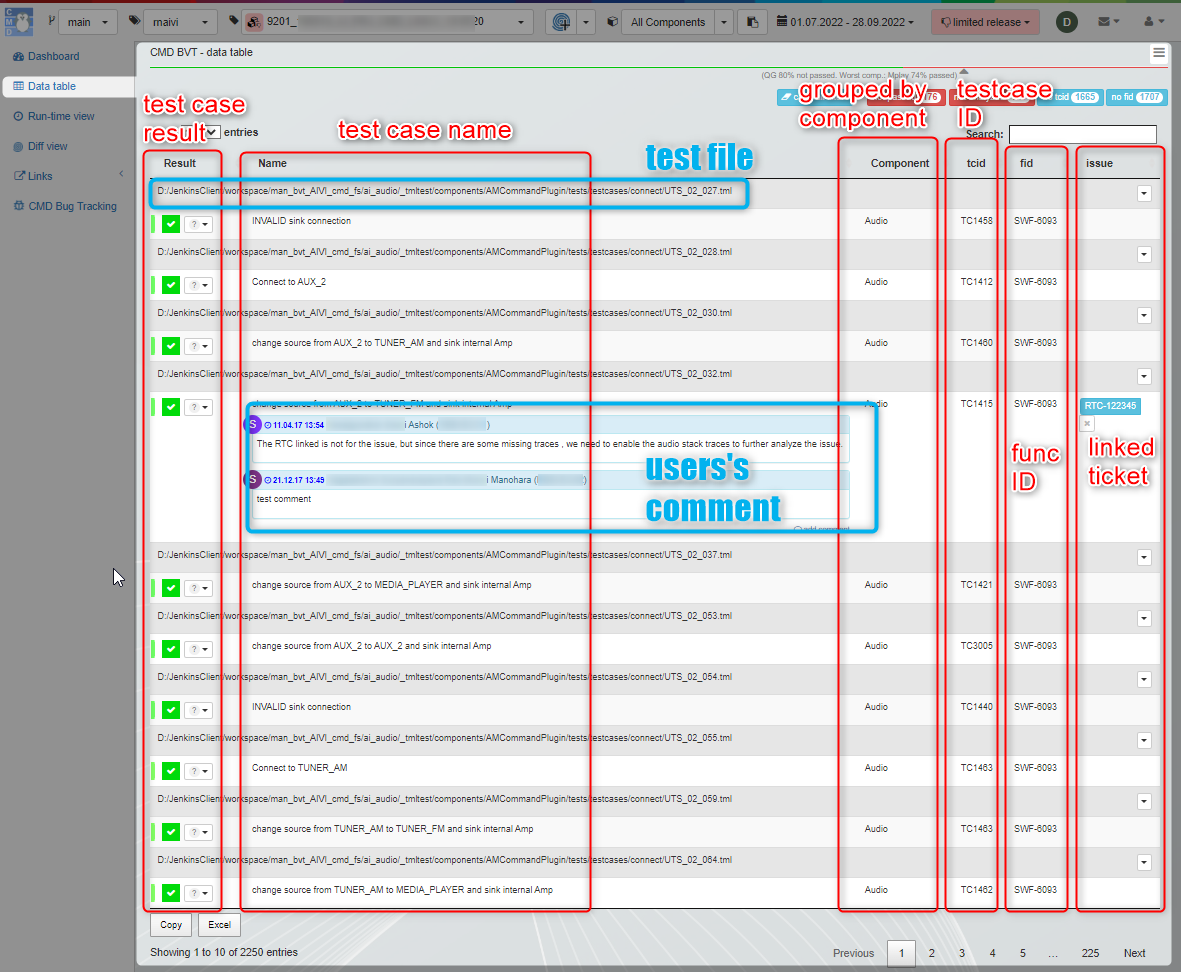
\includegraphics[width=1\linewidth]{./pictures/view_datatable.png}

Besides, you can aslo:
\begin{itemize}
   \item determine how many test cases (entries) are displayed in the table page.

         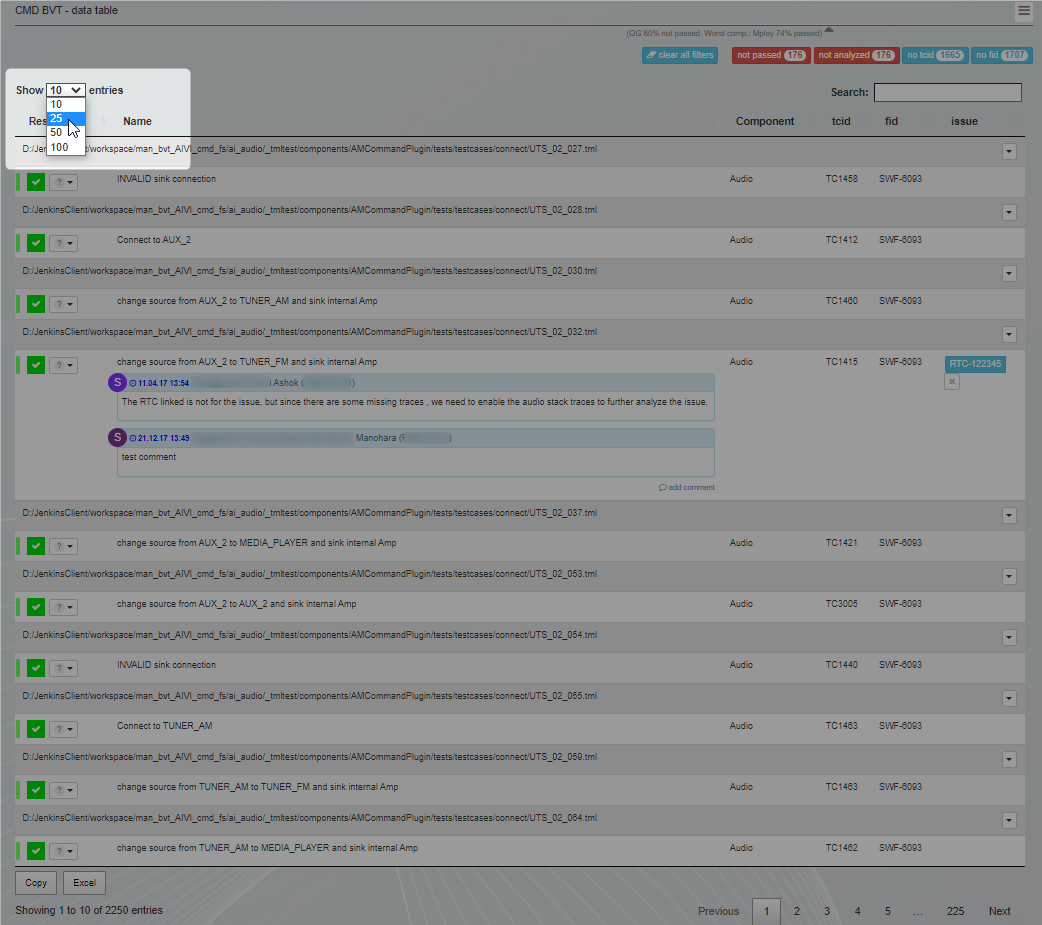
\includegraphics[width=0.6\linewidth]{./pictures/datatable/change_number_entries.png}
         
   \item apply filters to display such as not passed test cases.
   
         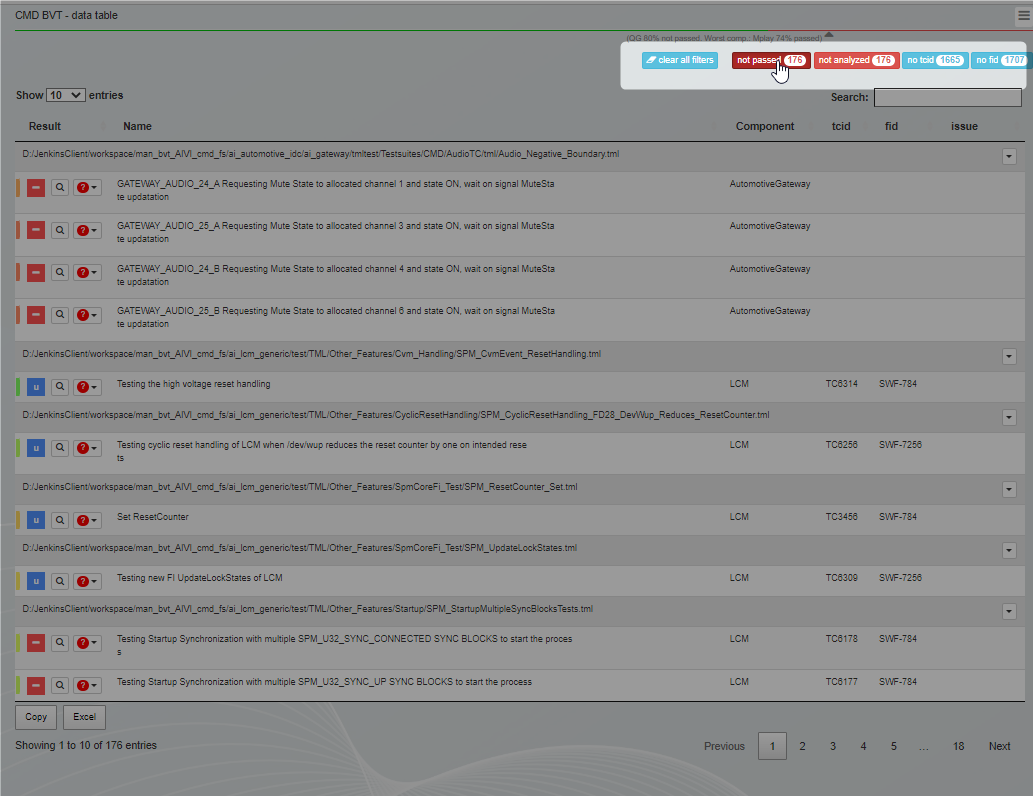
\includegraphics[width=0.6\linewidth]{./pictures/datatable/apply_filter.png}

   \item search for the specific test case for reference.
   
         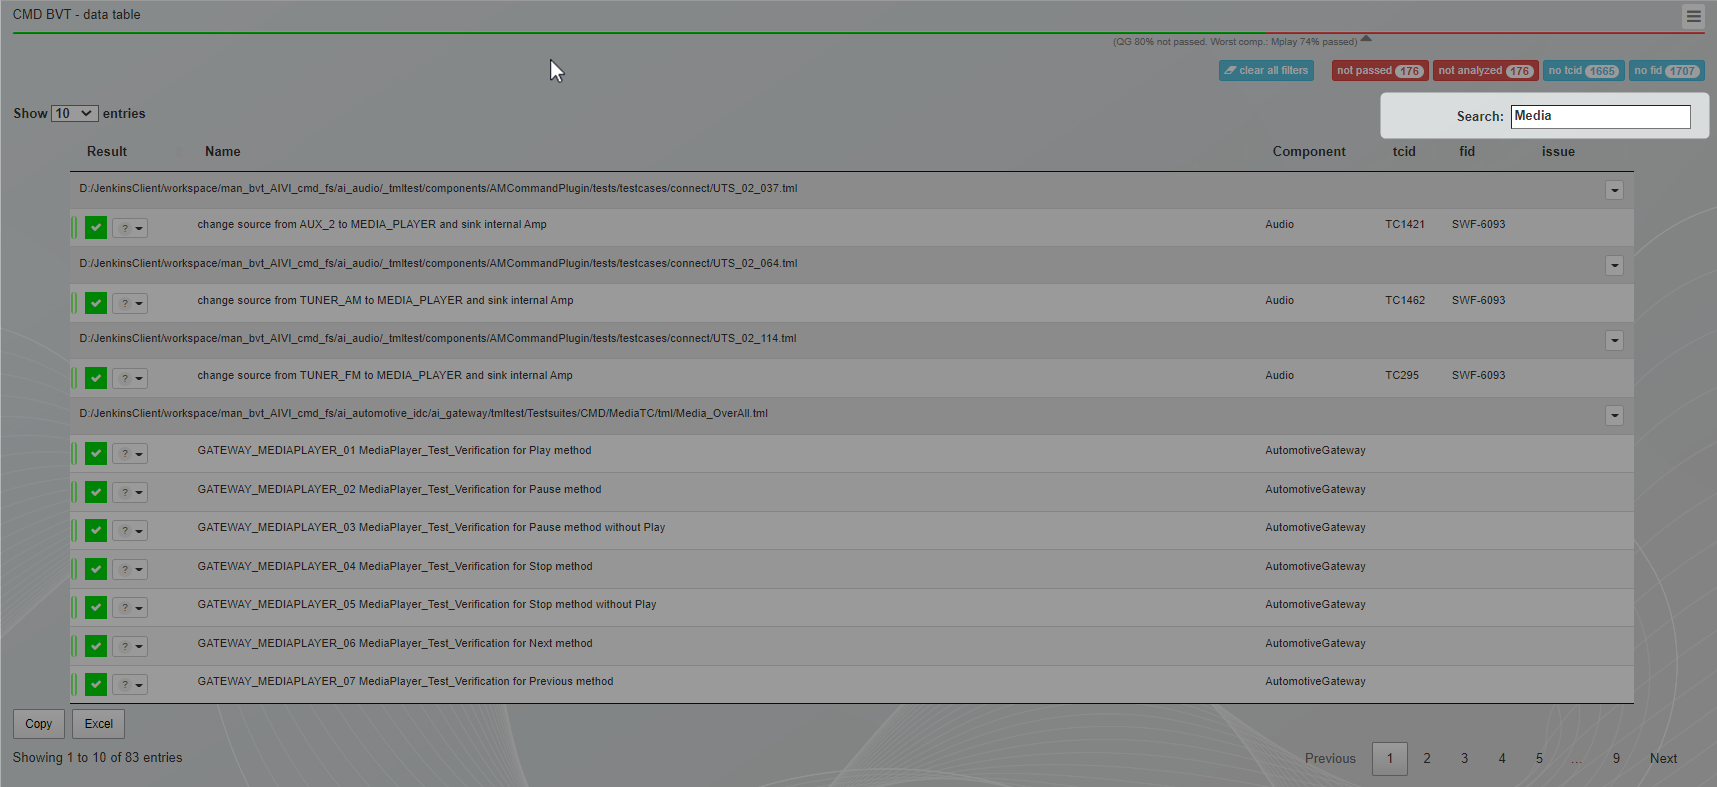
\includegraphics[width=0.6\linewidth]{./pictures/datatable/search.png}

   \item get more information about test environment, configurations.
   
         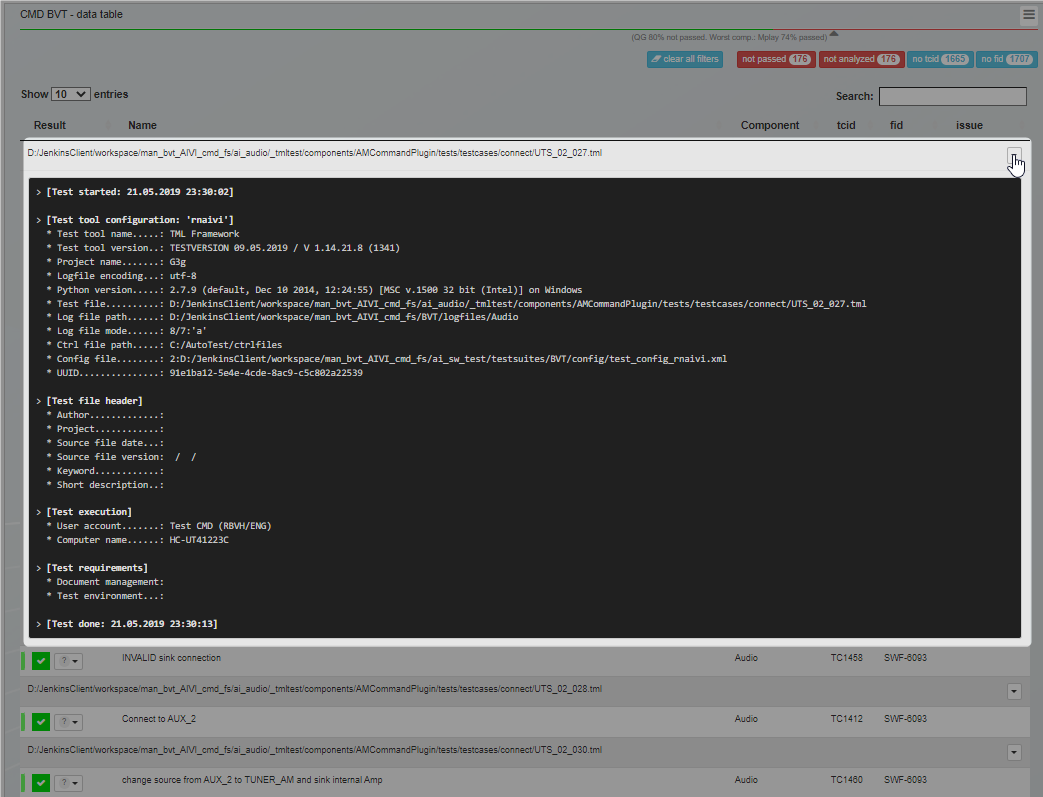
\includegraphics[width=0.6\linewidth]{./pictures/datatable/testcase_detail.png}

   \item get traceback information for not passed test case(s). An pop-up will 
         be displayed which show all record traceback (error) information.

         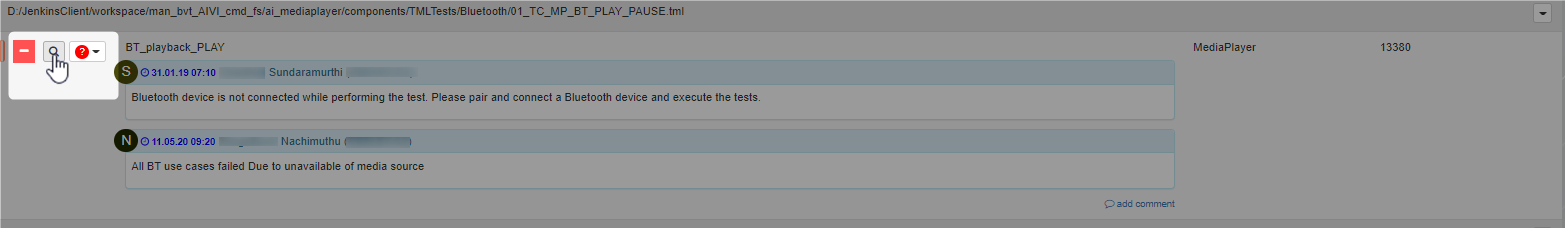
\includegraphics[width=0.6\linewidth]{./pictures/datatable/testcase_traceback.png}

   \item give comment to test case, link issue ticket to test case or observe
         the history of the user interaction on the test case.

         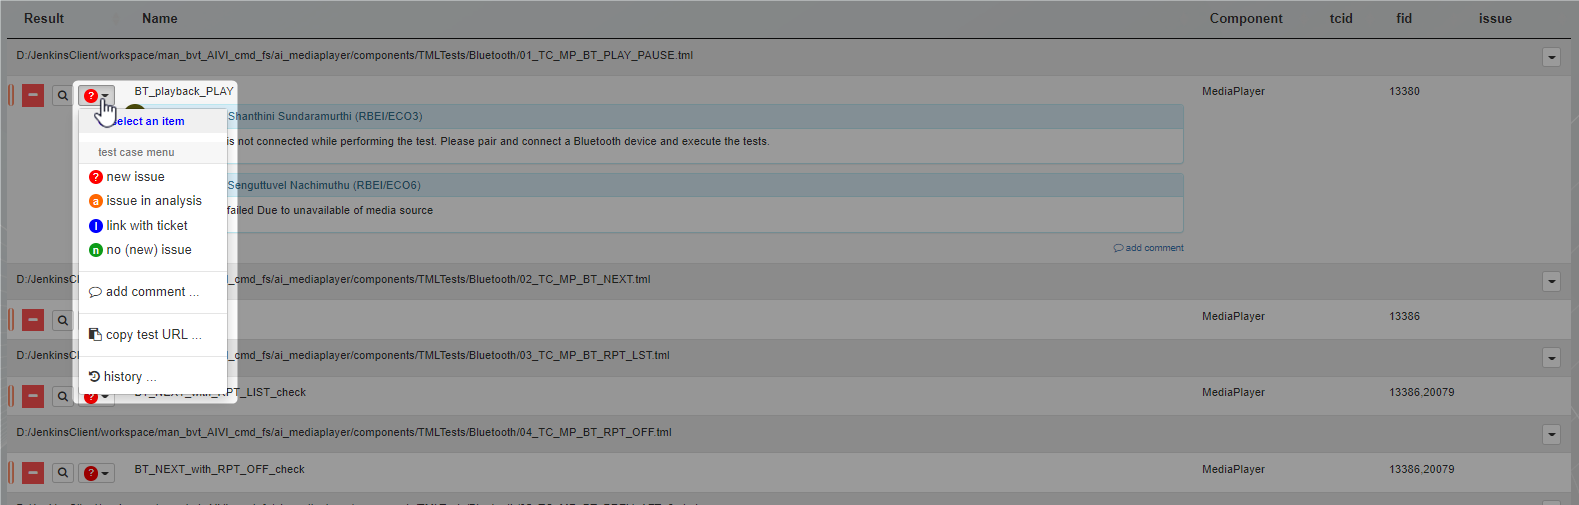
\includegraphics[width=0.6\linewidth]{./pictures/datatable/testcase_menu.png}

   \item copy data table or export them to the excel file.

         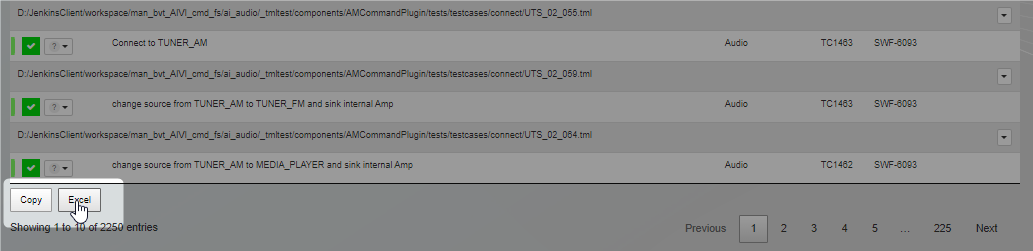
\includegraphics[width=0.6\linewidth]{./pictures/datatable/copy_export.png}
\end{itemize}


\hypertarget{runtime-view}{%
\subsection{Runtime View}\label{runtime-view}}
The runtime provides the treemap chart which helps you to know the time 
consumption of components within test execution result or test cases within
each component.

You can click on the component to go to detail run-time of all test cases within 
it and go back by clicking the component header.

With this view, you can understand run-time of a your test suite then optimize
the specific component or testcase if required.

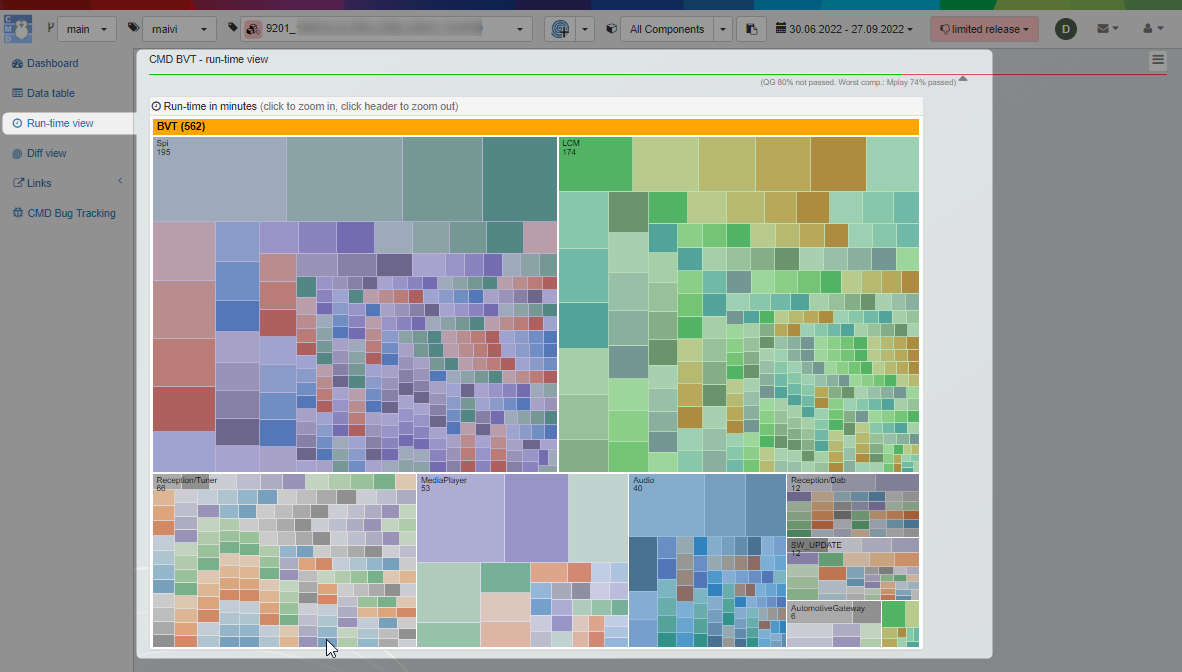
\includegraphics[width=1\linewidth]{./pictures/view_runtime.png}

\hypertarget{diff-view}{%
\subsection{Diff View}\label{diff-view}}
The diffview contains only the spiral chart which displays the differences 
between the software versions you want to compare. So that you can:
\begin{itemize}
   \item observe the test case result change (e.g from passed to failed).
   \item aware the new or removed test case(s).
   \item recognize the unstable test case(s)/component(s).
\end{itemize}

Be default, without adding the version for diffview, the current selected 
version and its around versions (the previous and the next version if existing) 
will be chosen for diffview as below:

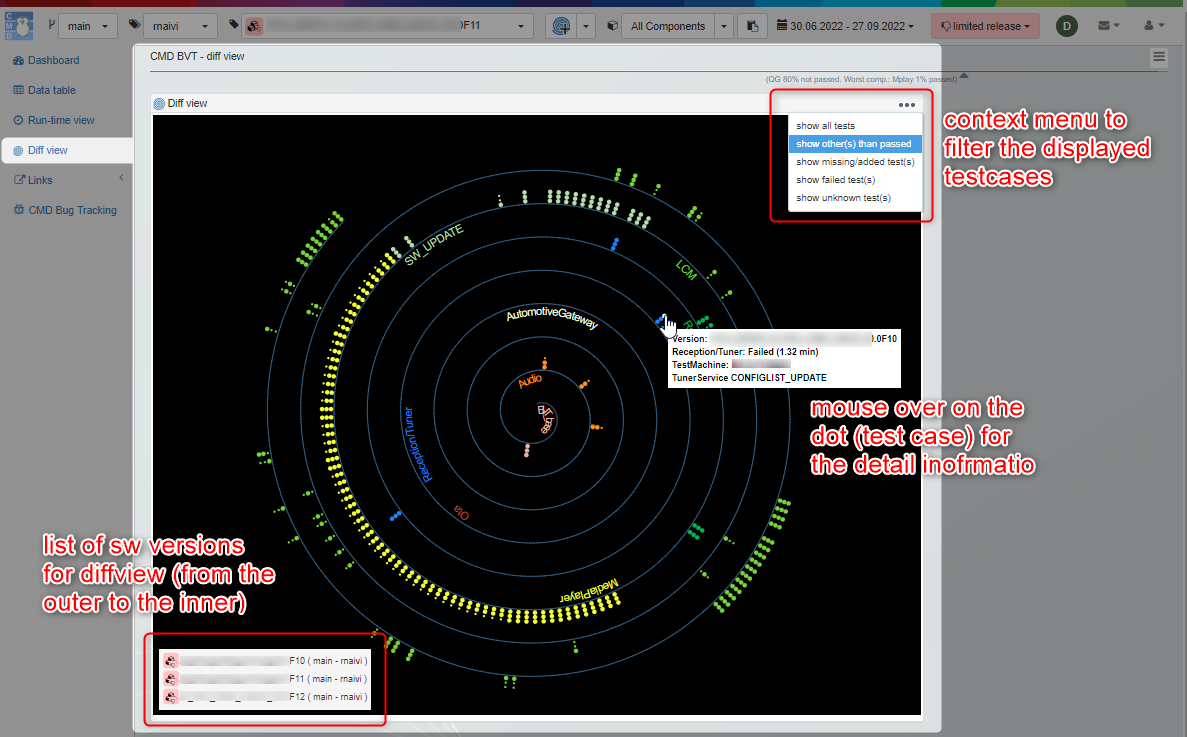
\includegraphics[width=1\linewidth]{./pictures/diffview/default_detail.png}

In case, you want to add the specific versions for diffview, select the version
from the version select box then click the add button 
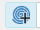
\includegraphics{./pictures/diffview/add_button.png} to add it to the list of 
diffview. 

The next dropdown button is used for viewing your selected version.
You can also clear your selection with \textbf{clear list} option.

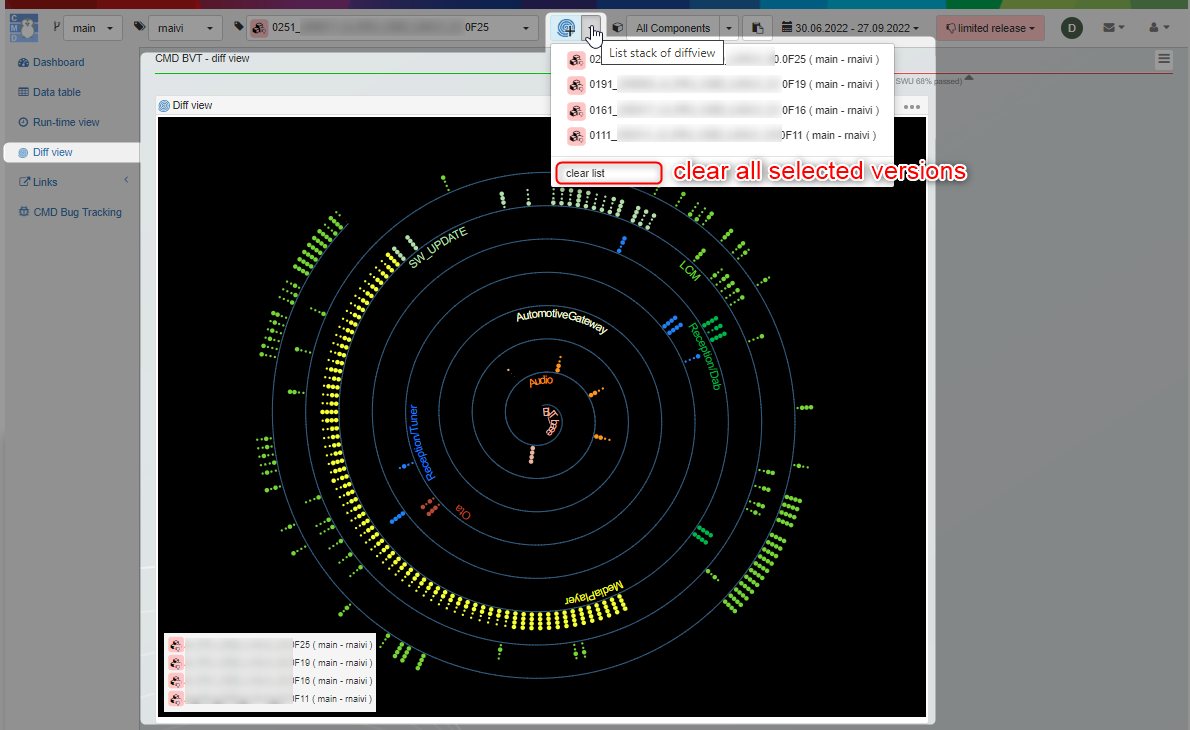
\includegraphics[width=1\linewidth]{./pictures/diffview/selected_version.png}

As soon as the new version is added for diffview, the spiral chart is updated 
immediately.

The dots which present for the test cases along the spiral line (small dot is 
passed and bigger one for other status) are interactable. It means that you can:
\begin{itemize}
   \item mouse over the dots to see the test case information.
   \item click on the failed test case (bigger dot) for the traceback informtion.
\end{itemize}

\begin{boxhint}{Notice:}
   You can only select maximum of \textbf{5} versions for diffview.

   If the maximum of selected versions is reached and you click on the button to 
   add more, the warning message will be displayed to prevent that action.
\end{boxhint}

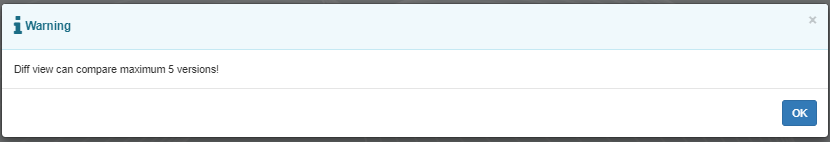
\includegraphics[width=1\linewidth]{./pictures/diffview/warning.png}